In this section we will present some preliminary results of our VM.
First, we present scalability results in order to show that LM programs take advantage of the advantages of multicore architectures.
Next, we present some absolute execution times and a comparison with similar programs in other programming languages.
We want to present evidence that LM is a viable language.

For our experimental setup, we used a machine 
with two 16 (32) Core AMD Opteron
(tm) Processor 6274 $@$ 2.2 GHz with 32 GBytes of RAM memory and running the Linux
kernel 3.8.3-1.fc17.x86\_64.
     We compiled our VM using GCC 4.7.2 (g++) with the flags \texttt{-O3 -std=c+0x -march=x86-64}.
     We run all experiments 3 times and then averaged the execution time.
     
\subsubsection{Scalability Results}

For this section, we run each program using 1, 2, 4, 6, 8, 10, 12, 14 and 16 threads and compared the runtime against the execution of the sequential version of the VM. We used the following programs:

\newcommand{\figsize}[0]{6.5cm}
\captionsetup[sub]{              % The subcaption settings
       font=scriptsize}

\begin{itemize}
   \item Greedy Graph Coloring (GGC) colors nodes in a graph so that no two adjacent nodes have the same color. We start with a small number of colors and then we expand the number of colors when we cannot color the graph.
   \item PageRank implements an asynchronous PageRank algorithm without synchronization between iterations. Every time a node sends a new rank to its neighbors and the change was significant, the neighbors are scheduled to recompute their ranks.
   \item N-Queens, the classic puzzle for a 13x13 board.
   \item Belief Propagation, a machine learning algorithm to denoise images.
\end{itemize}

Figure~\ref{exp:graph_coloring} presents the speedup results for the GGC program using 2 different datasets. In Fig.~\ref{exp:graph_coloring}~(a) we show the speedup for a graph of 12,000 webpages\footnote{The search engine graph was retrieved from \url{http://www.cs.toronto.edu/~tsap/experiments/download/download.html}}. Since this dataset follows the power law, that is, there is a small number of pages with a lots of links (1\% of the nodes have 75\% of the edges), the speedup is slightly worse than the benchmark shown in Fig.~\ref{exp:graph_coloring}~(b), where we use a random dataset of 2,000 nodes and an uniform distribution of edges.

\newcommand{\plotsize}{0.38\textwidth}

\begin{figure*}[h]
   \vspace{-0.5\intextsep}
   \centering
   \begin{subfigure}[b]{\plotsize}
      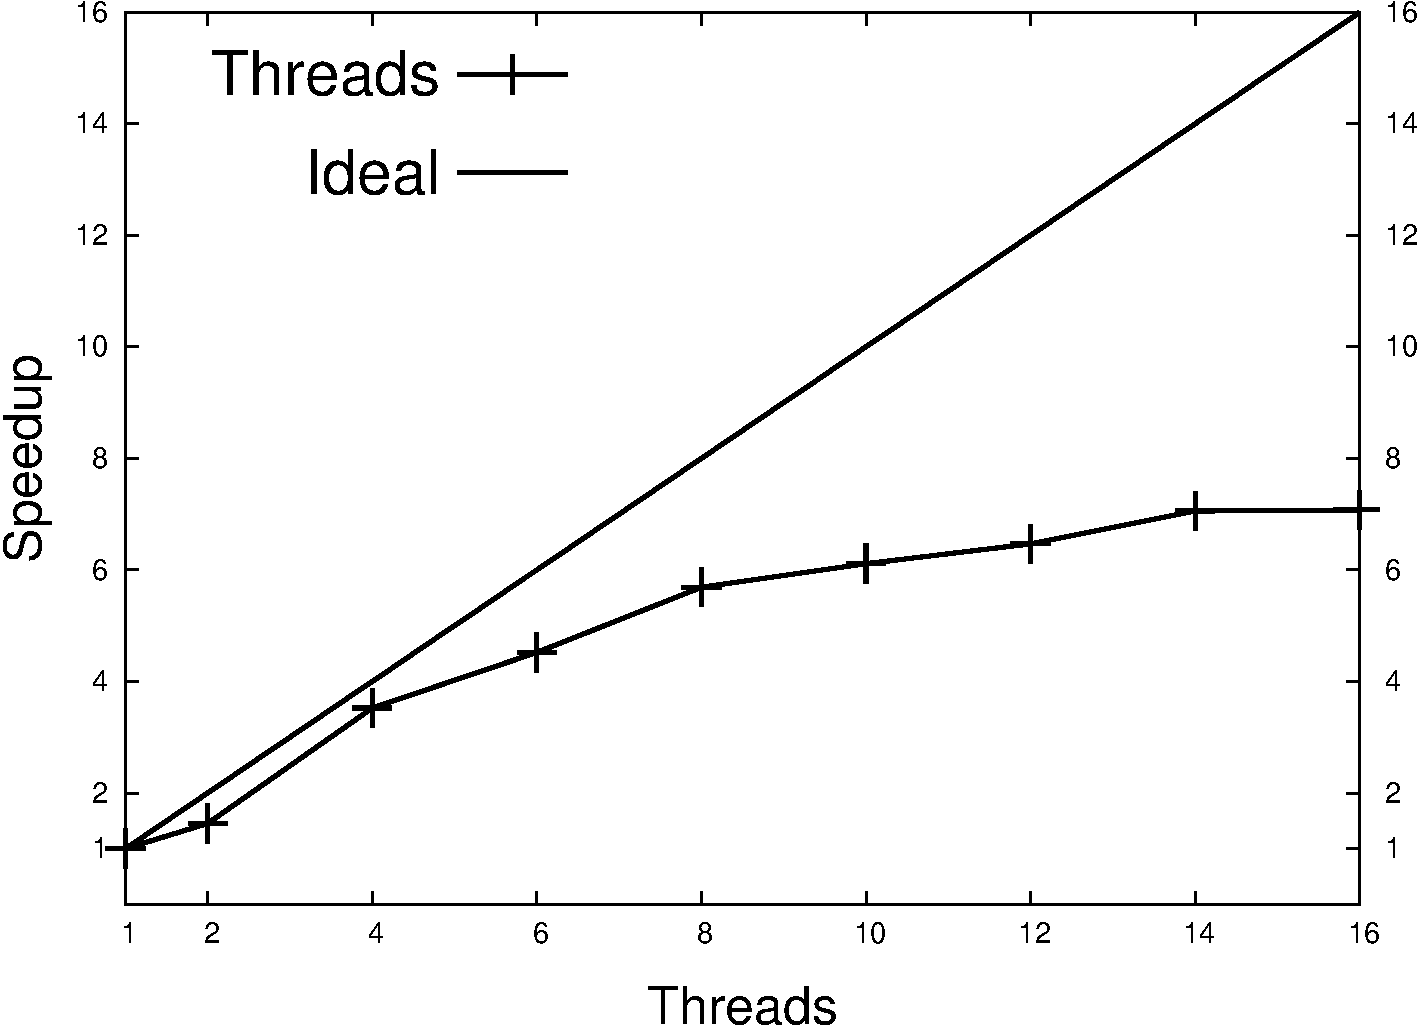
\includegraphics[width=\textwidth]{speedup_greedy-graph-coloring-search_engines.pdf}
      \caption{Using a graph of web pages collected from a search engine (around 12,000 nodes and 292,000 edges).}
   \end{subfigure}
   \begin{subfigure}[b]{\plotsize}
      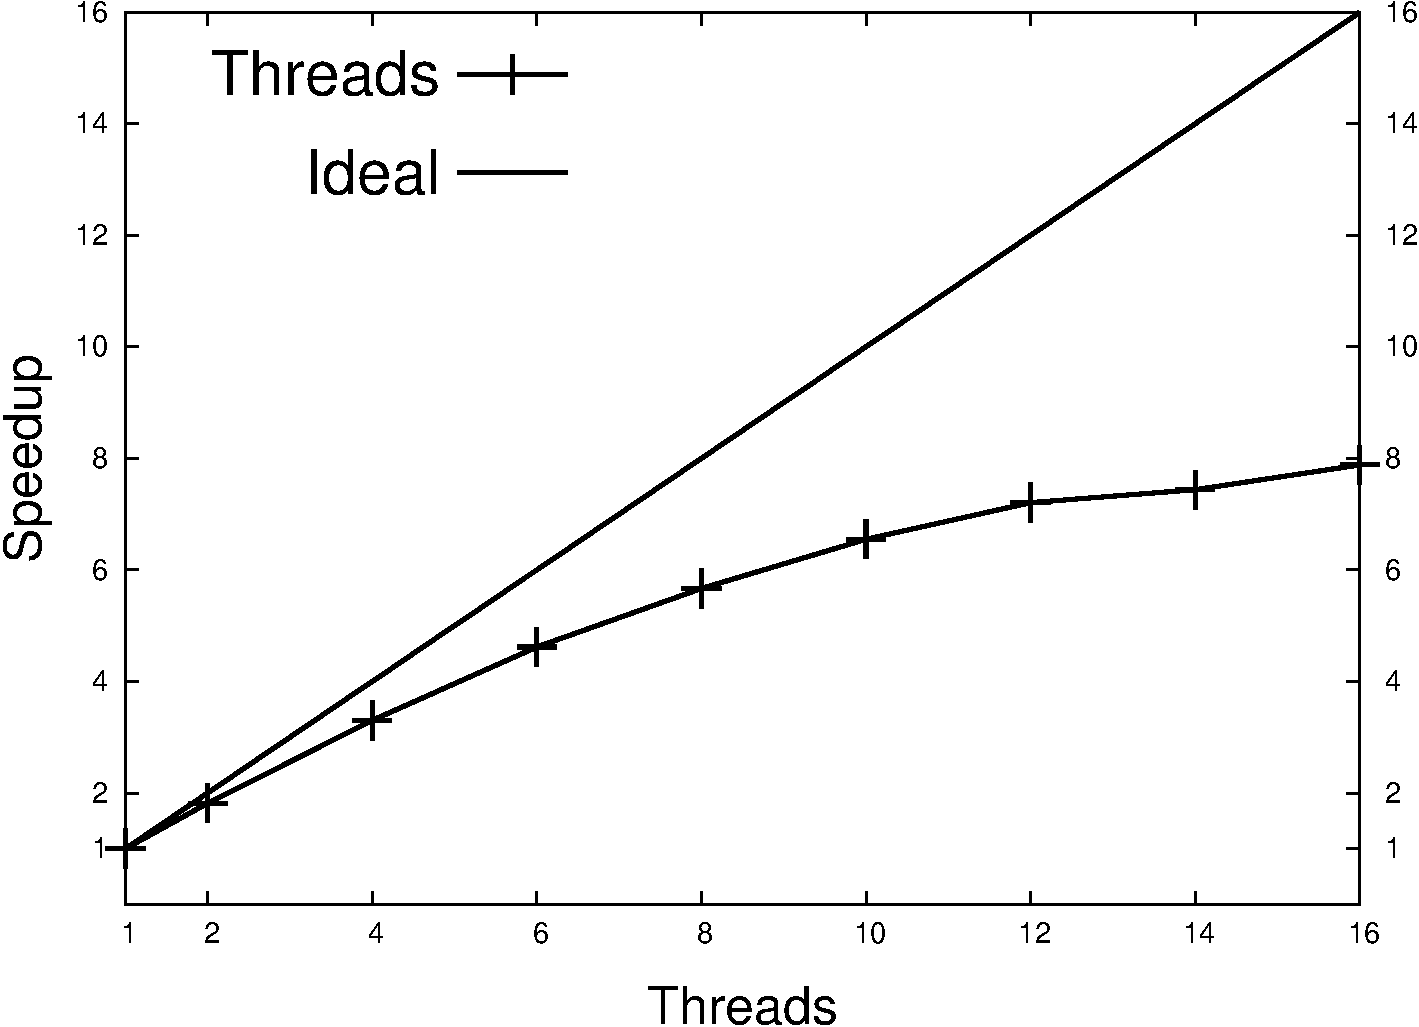
\includegraphics[width=\textwidth]{speedup_greedy-graph-coloring-2000.pdf}
      \caption{Using a random graph with 2,000 nodes and 600,000 edges.\newline}
   \end{subfigure}
   \caption{Experimental results for the GGC algorithm.}
   \label{exp:graph_coloring}
   \vspace{-0.8\intextsep}
\end{figure*}

The PageRank results are shown in Fig.~\ref{exp:pagerank}. We used the same search engine dataset as before and a new random dataset with 5000 nodes and 500,000 edges. Although the search engine graph (Fig.~\ref{exp:pagerank}~(a)) has half the edges (around 250,000), it scales better than the random graph (Fig.~\ref{exp:pagerank}~(b)), meaning that the PageRank program depends on the number of nodes to be more scalable.

\begin{figure*}[h]
   \vspace{-0.5\intextsep}
   \centering
   \begin{subfigure}[b]{\plotsize}
      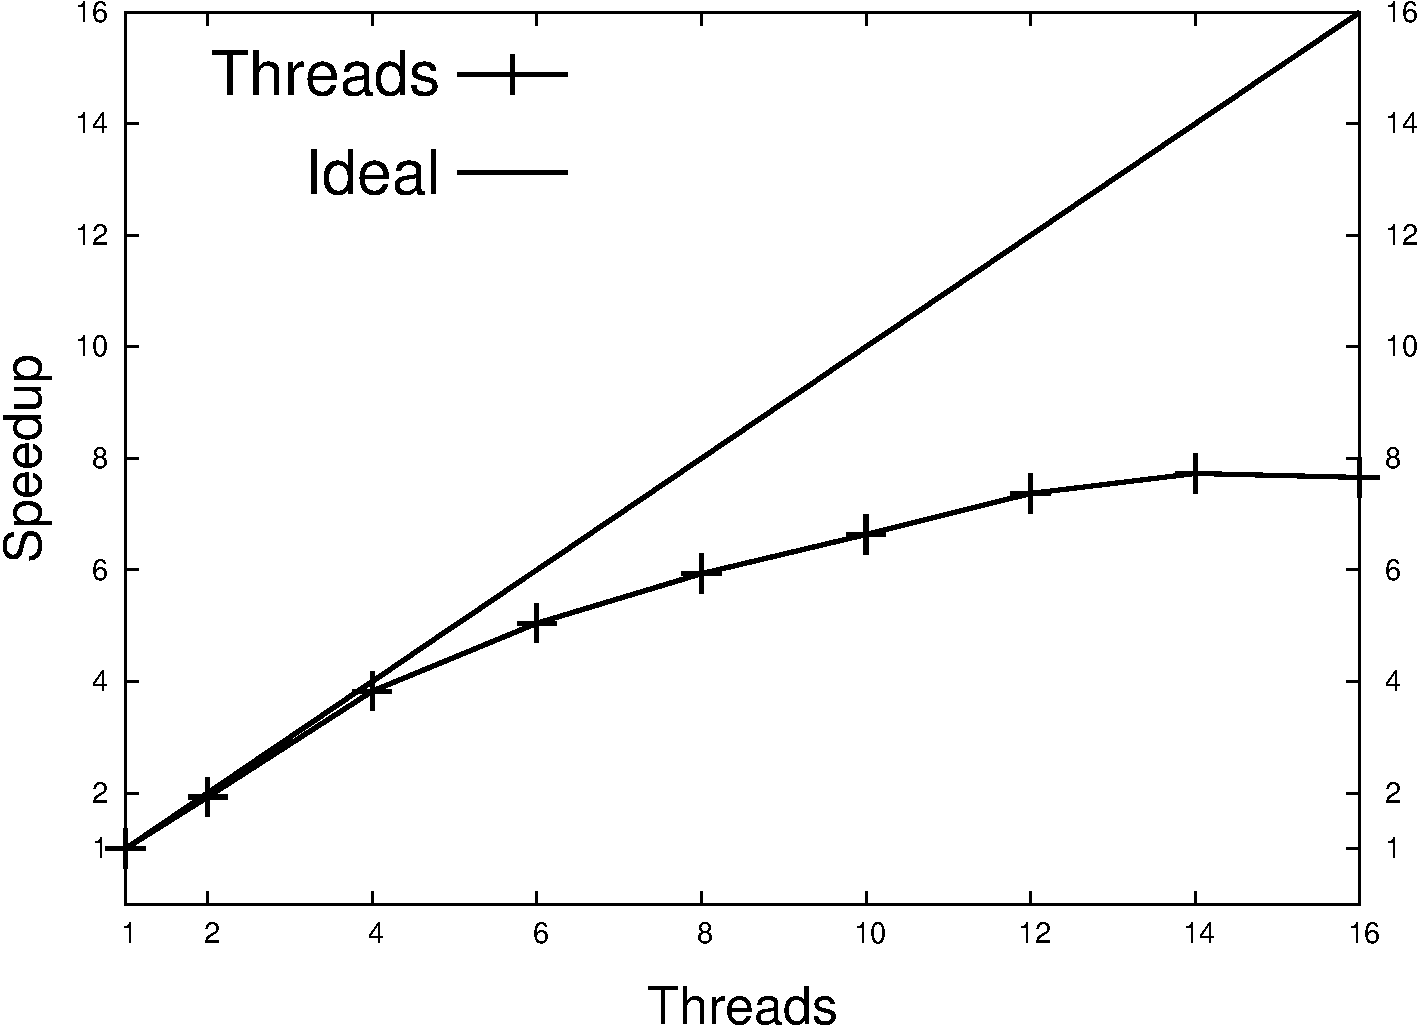
\includegraphics[width=\textwidth]{speedup_pagerank-search_engines.pdf}
      \caption{Using a graph of web pages collected from a search engine (around 12,000 nodes and 292,000 edges)}
   \end{subfigure}
   \begin{subfigure}[b]{\plotsize}
      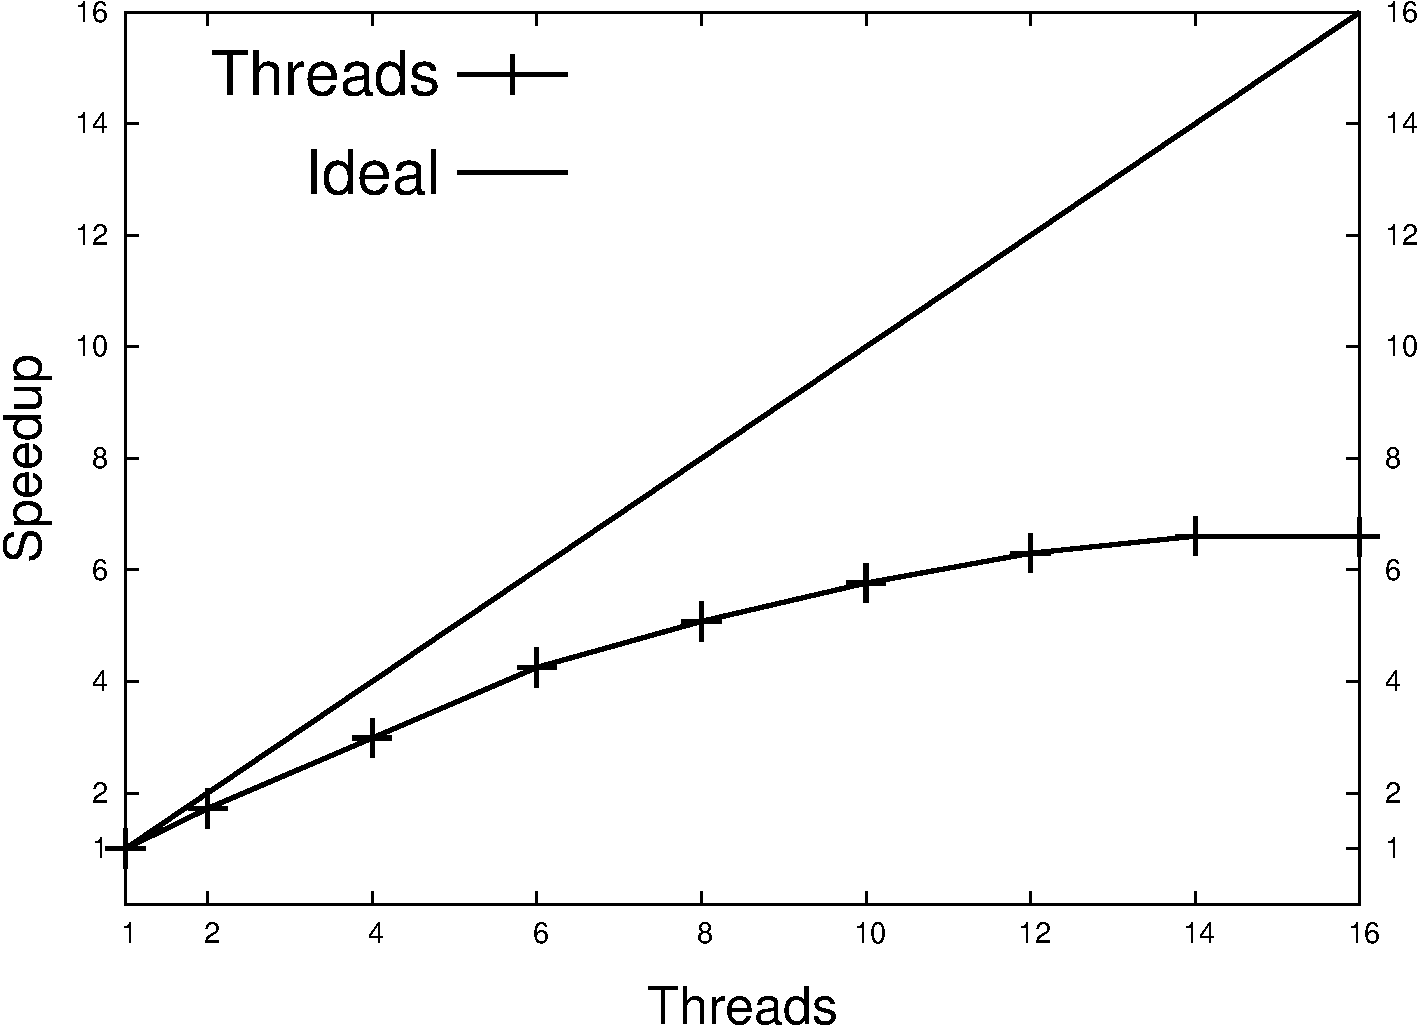
\includegraphics[width=\textwidth]{speedup_pagerank-5000.pdf}
      \caption{Using a random graph with 5,000 nodes and 500,000 edges.\newline}
   \end{subfigure}
   \caption{Experimental results for the asynchronous PageRank algorithm.}
   \label{exp:pagerank}
   \vspace{-0.8\intextsep}
\end{figure*}

\begin{figure*}[h]
   \vspace{-0.5\intextsep}
   \centering
   \begin{subfigure}[b]{\plotsize}
      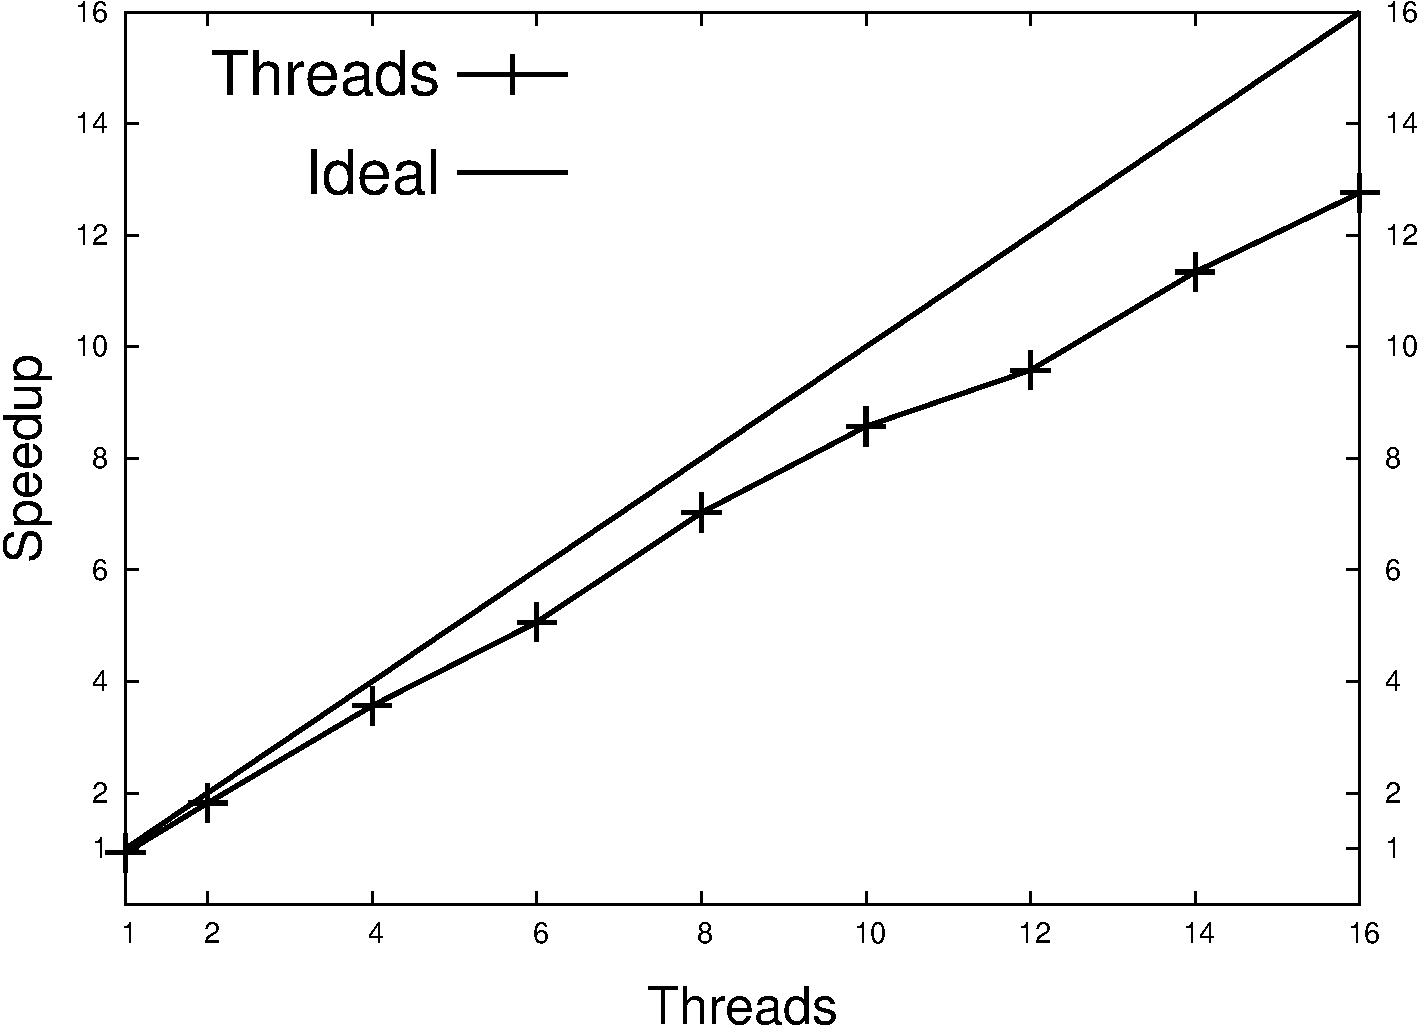
\includegraphics[width=\textwidth]{speedup_8queens-13.pdf}
      \caption{N-Queens program (13x13~board).}
      \label{exp:8queens}
   \end{subfigure}
   \begin{subfigure}[b]{\plotsize}
      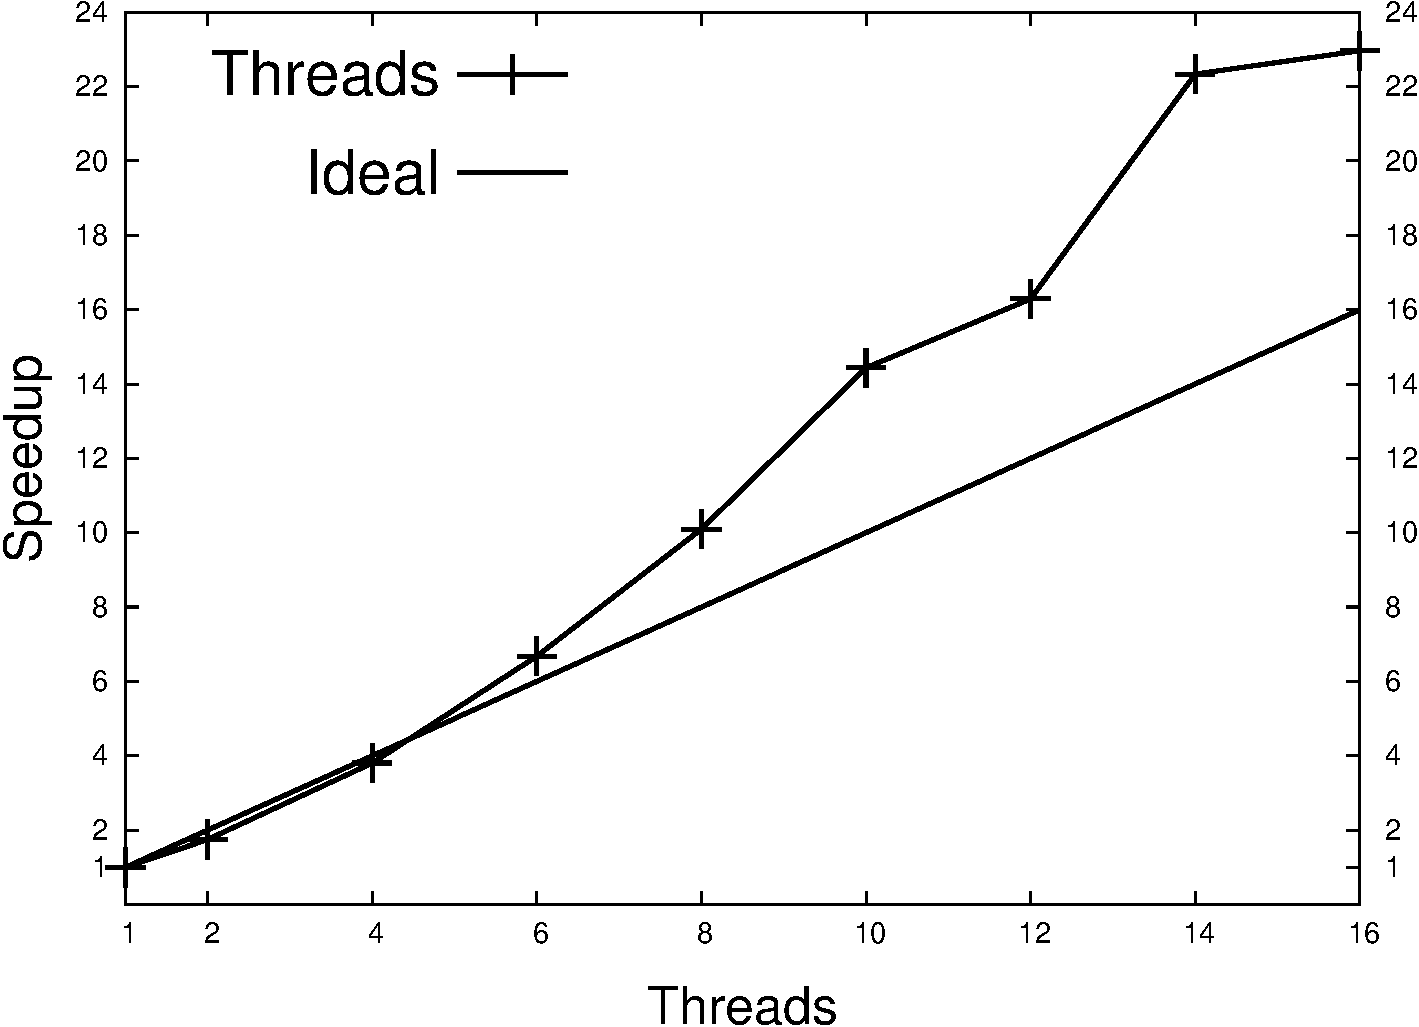
\includegraphics[width=\textwidth]{speedup_bp-400.pdf}
      \caption{BP (400x400~image).}
      \label{exp:bp}
   \end{subfigure}
   \caption{Experimental Results for N-Queens and Belief Propagation.}
   \vspace{-0.8\intextsep}
\end{figure*}

The results for the N-Queens program are shown in Fig.~\ref{exp:8queens}. The program is not regular since computation starts at the top of the grid and then rolls down, until only the last row is doing computation. Because the number of valid states for the nodes in the upper rows is much less than the nodes in the lower rows, this may create potential load balancing problems. The results show that our system is able to scale well due to work stealing.

Finally, we shown the results for the Belief Propagation~(BP) program in Fig.~\ref{exp:bp}. BP is a regular and asynchronous program
and benefits (as expected) from having multiple threads executing since the belief values of each node will converge faster.
The super-linear results prove this assertion.

\subsubsection{Absolute Execution Time}

As we have seen, our VM scales reasonably well, but how does it fair in terms of absolute execution time? We now compare the execution
time using one thread against other competing systems.

In Fig.~\ref{comp:nqueens} we compare the LM's N-Queens version against 3 other versions: a straightforward sequential program implemented
in C using backtracking; a sequential Python~\cite{vanRossum:1995:PRM} implementation; and a Prolog implementation executed in
YAP Prolog~\cite{DBLP:journals/corr/abs-1102-3896}, an efficient implementation of Prolog. Numbers less than 1 mean that LM
is faster and larger than 1 mean that LM is slower. We see that LM easily beats Python, but is 5 to 10 times slower than YAP
and around 15 times slower than C.
However, note that if we use at least 16 threads in LM, we can beat the sequential implementation written in C.

\begin{figure*}[h]
   \vspace{-0.2\intextsep}
   \centering
   
   \begin{subfigure}[b]{0.45\textwidth}
      \resizebox{5cm}{!} {
      \begin{tabular}{ | l | l | l | l |}
       \hline

       Size & C & Python & YAP Prolog \\ \hline\hline
       10 & 16.92 & \textbf{0,62} & 5,42 \\
       11 & 21.59 & \textbf{0.64} & 6.47 \\
       12 & 10.32 & \textbf{0.73} & 7.61 \\
       13 & 14.35 & \textbf{0.88} & 10.38 \\
       \hline
       \end{tabular}}
       \caption{N-Queens problem.}
      \label{comp:nqueens}
   \end{subfigure}
   \begin{subfigure}[b]{0.45\textwidth}
      \resizebox{4.6cm}{!} {
      \begin{tabular}{ | l | l | l | l |}
       \hline

       Size & C & Python & GraphLab \\ \hline\hline
       10 & \textbf{0.67} & \textbf{0,03} & \textbf{1.00} \\
       50 & \textit{1.77} & \textbf{0.04} & \textit{1.73} \\
       200 & \textit{1.99} & \textbf{0.05} & \textit{1.79} \\
       400 & \textit{2.00} & \textbf{0.04} & \textit{1.80} \\
       \hline
       \end{tabular}}
       \caption{Belief Propagation program.}
       \label{comp:bp}
   \end{subfigure}
   \caption{Comparing absolute execution times (System Time / LM Time).}
   \vspace{-0.8\intextsep}
\end{figure*}

In Fig.~\ref{comp:bp} we compare LM's Belief Propagation program against a sequential C version, a Python version and a GraphLab version. GraphLab~\cite{GraphLab2010} is a parallel C++ library used to solve graph-based problems in machine learning. C and GraphLab
perform about the same since both use C/C++. Python runs very slowly since it is a dynamic programming language and BP has many
mathematical computations. We should note, however, that the LM version uses some external functions written in C++ in order
to improve execution time, therefore the comparison is not totally fair.

We also compared the PageRank program against a similar GraphLab version and LM is around 4 to 6 times slower.
Finally, our version of the all-pairs shortest distance algorithm is 50 times slower than a C sequential implementation of the Dijkstra algorithm, but it is almost twice as fast when compared to the same implementation in Python.